\documentclass{article}
\usepackage{tikz}
\usetikzlibrary{arrows.meta,positioning,calc,shapes.geometric}
\pagestyle{empty}
\begin{document}
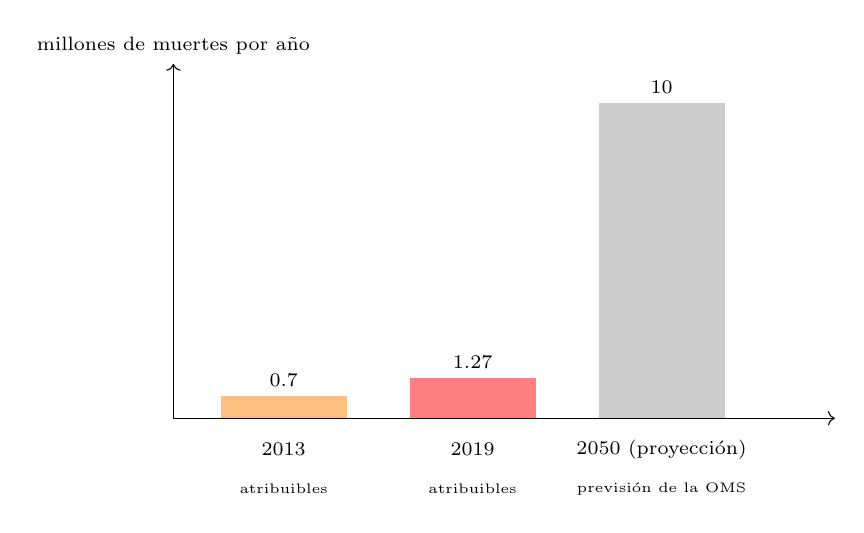
\begin{tikzpicture}

\def\bar#1#2#3{\fill[#3] (#1,0) rectangle (#1+1.6,{#2*0.4}); \node[font=\scriptsize, above] at (#1+0.8,{#2*0.4}) {#2};}
\draw[->] (0,0) -- (0,4.5) node[above, font=\scriptsize] {millones de muertes por año}; \draw[->] (0,0) -- (8.4,0);
\bar{0.6}{0.7}{orange!50}\bar{3.0}{1.27}{red!50}\bar{5.4}{10}{gray!40}
\node[font=\scriptsize] at (1.4,-0.4) {2013}; \node[font=\scriptsize] at (3.8,-0.4) {2019}; \node[font=\scriptsize] at (6.2,-0.4) {2050 (proyección)};
\node[font=\tiny, align=center] at (1.4,-0.9) {atribuibles}; \node[font=\tiny, align=center] at (3.8,-0.9) {atribuibles}; \node[font=\tiny, align=center] at (6.2,-0.9) {previsión de la OMS};

\end{tikzpicture}
\end{document}
